%% ------------------------------------------------------------------------- %%
\chapter{Hash Functions}
\label{cap:Hash Functions}

%% ------------------------------------------------------------------- %%
%\begin{itemize}
%\item Define Hash Function
%\item Give some examples of hash functions (Multiplicative / Remainder)
%\item Present Dragon Book metric and Evaluate hash functions
%\end{itemize}
%% ------------------------------------------------------------------- %%

Outside computer science, the word \textit{``hash''} in the english language means to ``chop'' or to ``mix'' something. This meaning is entirely related to what hash functions are supposed to do. hash functions are functions that are used to map data of an arbitrary size to data of a fized size \cite{HashFuncWiki}.

They have wide applications in computer science, being used in information and data scurity, compilers, distributed systems and hardcore algorithms. During this chapter I first define and explain the basics of a hash function, then I give an intiution in some metrics of what is a good hash function, as discussed in the famous \textit{``Red Dragon Book''} \cite{DragonBook} along with some reproduction of known results in the area.

The value extracted from the hash function for an object is usually called \textit{Hash Value}. The hash value is usually, but not necessarily, smaller than the object that generated it. For example, we can have a hash function that takes Gigabytes or Terabytes files and return an 8 bytes hash value.

\begin{figure}[h!]
  \centering
  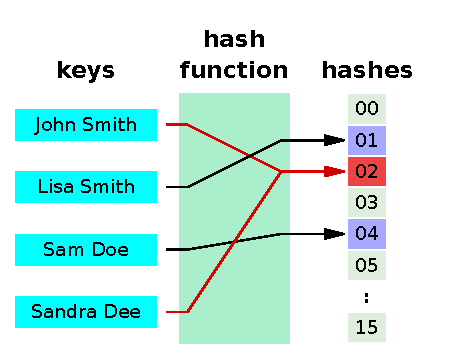
\includegraphics[width=10cm]{figuras/hash-function.pdf}
  \caption{Example of a hash function from string to 4 bit integer. }
\end{figure}

\bigskip

To formalize a little, lets define a hash function as a function \( H \) that takes an element \( x \in X \) and has \( [0, M) \) as a codomain.

This is the same definition used by Donald Knuth \cite{TAOCP3} and some articles \cite{RobinHoodHashing}. This definition makes sense for our case because we will be talking mostly about hash functions used in hash tables, and in that case we want integers that will be indexes in an array (as we will se later on). In other cases will may see hash functions value as strings, like for when we hash an string for password storage or when we use a hash function in files for check-sum (for when we are checking if two files are the same). For the goal of this thesis we will not be focusing on those functions, but it is important to notice that strings can also be abstracted to integers if we just look at the bytes.

For our specific case we are looking at a hash function that is good for the construction of hash tables, that is that is fast to calculate and minimizes the number of collisions. Depending on our goals we might want a different metric, for check-sums for example we may want a function that is very sensible to chages, and for passwords one that is very hard to find its inverse.

As said in Donald Knuth's book, we know that it is theoricatically impossible to create a hash functio that generates true random data from non random data in actual file, but we can do pretty close to that (or in some cases, even better).  Donald Knuth describes 2 specific methods for simple hash function, named \textit{division hashing} and \textit{multiplicative hashing} techniques. As the name sugests, the first is based on division and the former on multiplication.

The divison hashing method simply to represent the data as a number take the remainder of that number modulo a value. Supposing that we can represent the data as a non negative integer \( X \) the division hashing would be to choose a value M and the hashing function would be \( X mod M \). The C++14 code would look as following:

\begin{lstlisting}
unsigned_int divisionHashing(unsigned_int X, unsigned_int M) {
  return X % M;
}
\end{lstlisting}

In general large prime numbers tend to be a good value to \( M \), because if not we may have repetitions. One great example of this is if \( M \) is even, then the parity of hash value of \( X \) will match the parity of \( X \) (which will cause a bad distribution). The same pattern will happen in different intervals for different powers of \( 2 \).

For the multiplicative hashing, we can furst imagine that the overflow is like a ``natural'' modulo operation (We also have methods to take the modulo without overflowing, to know more about that ). Supposing that we can represent the data as an non negative integer \( X \), the multiplication hashing would be to choose a value \( A \) that we mulitply by \( X \) and then take the value module \( 2^P \) (That is how is described in donald knuth book, by \textit{``taking the leading bits of the least signifcant half of \( A * X \)''}). The C++14 code would look as follwing:

\medskip

\begin{lstlisting}
unsigned_int multiplicativeHashing(unsigned_int X,
                                   unsigned_int A,
                                   unsigned_int P) {
  return (A * X) << P; 
}
\end{lstlisting}

In knuth's book he restricts \( A \) to be relatively prime to \( w \), being \( w \) the size of a ``word'' in the machine (which is \( MAX\_INT \) in our case). That definition is often useful if you can retrieve a value \( Y \) for a given hash value \( F \). It is good to note here that if \( H(X) = F \) and \( H(Y) = F \), \( X \) is not necessarily equal to \( Y \), as two keys can have the same hash value.

Here it is also good to note, we have many ways of converting non numerical data to non negative integers. In the end, it is all just a sequence bytes, that when readed in a specific way form another type of data, such as images or strings. For example, one way of transforming a string to a non negative integer is summing the ASCII value of its characters. The C++14 code for that would look as following:

\begin{lstlisting}
unsigned_int convertStringToInteger(string str) {
  unsigned_int hashValue = 0;
  for (char c : str) {
    hashValue += (int) c;
  }
  return hashValue;
}
\end{lstlisting}

We always use usigned integers for our non negative integer calculations due to the natural modulo operation of it on overflow cases. It is equivalent to having a \( mod \ 2^{32} \) every time it overflows (As we only look at the leading 32 bits). We can also use \( XOR \) function to mix numbers together. 

There is also a very common type of hash functions that tend to work pretty well for strings \cite{DragonHashFunc}. It is a ``Superset'' of multiplicative hash functions, or a generalization. The C++14 code would look as following:

\begin{lstlisting}
unsigned_int hashForString(string str,
                           unsigned_int initialValue,
                           unsigned_int multiplier,
                           unsigned_int modulo) {
  unsigned_int hash = initialValue;
  for (char c : str) {
    hash = (multiplier * hash + (int)c);
  }
  return hash % modulo;
}
\end{lstlisting}

The above function is very common for string hashing, and by just choosing a different initial value and multiplier we can have completely different hash funcitons. Although using summing or using XOR usually don't provide much difference, XOR is preferable due to the fact that we do not need to worry about overflow. Some values are of known hash funcitons, for example with \( multiplier = 33 \) and \( initialValue = 5381 \) generates \textit{Bernstein hash djb2} \cite{BernsteinHash} or \( multiplier = 31 \) and \( initialValue = 0 \) generates \textit{Kernighan and Ritchie's hash} \cite{KernighanHash}. Those are famous functions and their values are not choosen randomly, as there are some factors that maximizes the chance of producing a good hash function (remembering, good means low collision rate and fast computation). Those factors are:

\begin{itemize}
\item The multiplier should be bigger than the size of your alphabet (in our case usually 26 for english words or 256 for ASCII). That is the case because if it is smaller we can have wrong matches easier. For example, suppose that \( multiplier = 10 \) and \( initialValue = 0 \), we have \( H('ABA') = H('AAK') = 7225 \) before taking the modulo operation.

\item The multiplication by the multiplier should be easy to calculate with simple operations, such as bitwise operations and adding. That is quite intuitive as we want a hash function that is fast to calculate. 

\item The multiplier should be coprime with the modulo. That is because if not we will ``cicle'' hashes at a greater rate than the modulo (We can use some modular arithmetic to prove that). Usually prime numbers tend to be good multipliers.
\end{itemize}

Now that we know some good templates for producing hash functions lets try to find a concrete metric or formula that measures the quality of a hash function. Fortunately, the famous Red Dragon Book \cite{DragonBook} has already proposed a formula to measures the quality of a hash function. The formula is the following:

\[ \sum_{j = 0}^{m - 1} \frac{b_j(b_j + 1)/2}{ (n/2m)(n + 2m - 1) } \]

Where \( n \) is the number of keys, \( m \) is the number of total slots and \( b_j \) is the number of keys in the \( j-th \) slot. The intuition for the numerator is the number of operations we will need to execute to find each element of the table. For example, we need 1 operation to find the first element, 2 to find the second, and so on. That means that we will end up with the follwing arithmetic progression. We know that a hash function that distributes the keys in a uniformly random distribution has expected bucket size of \( n / m \), so we can calculate that the expected value of the numerator formula is \( (n/2m)(n + 2m - 1) \). So that gives us a ratio of collisions (thinking just about operations to access a value) of ``our'' hash function with an ``ideal'' function. That means that a value close to \( 1.00 \) of the above formula is good, and values below to \( 1.00 \) means that we had less conflicts than an uniformly distributed random function.

From common data as used in Dragon Book and Strchr website \cite{DragonHashFunc} I will reproduce some tests with the previously cited hash functions.

\begin{figure}[h!]
  \raggedleft
  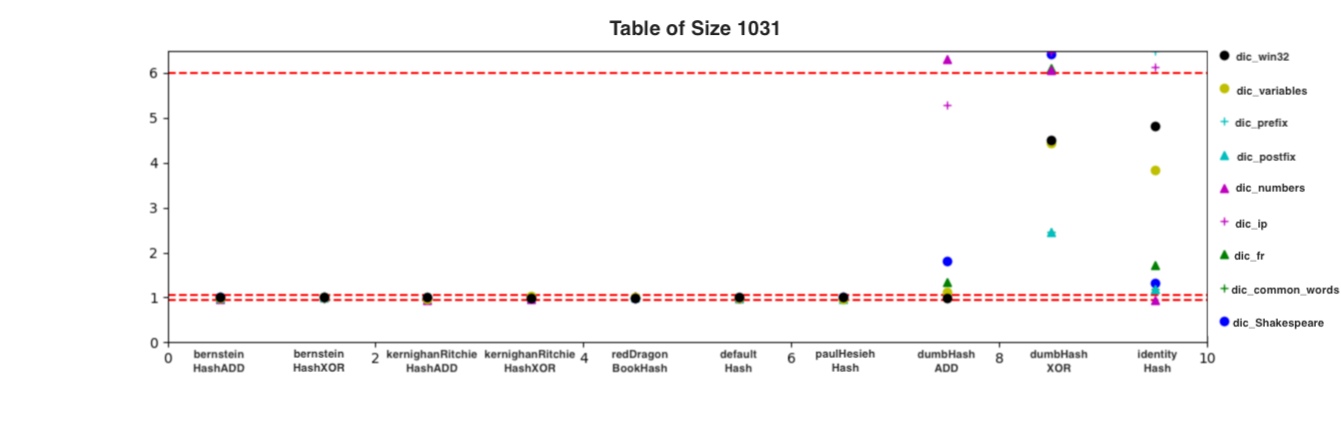
\includegraphics[width=18cm]{figuras/1031HashFunc.png}
  \caption{Functions tested against a ``small'' table}
\end{figure}

\medskip

\begin{figure}[h!]
  \raggedleft
  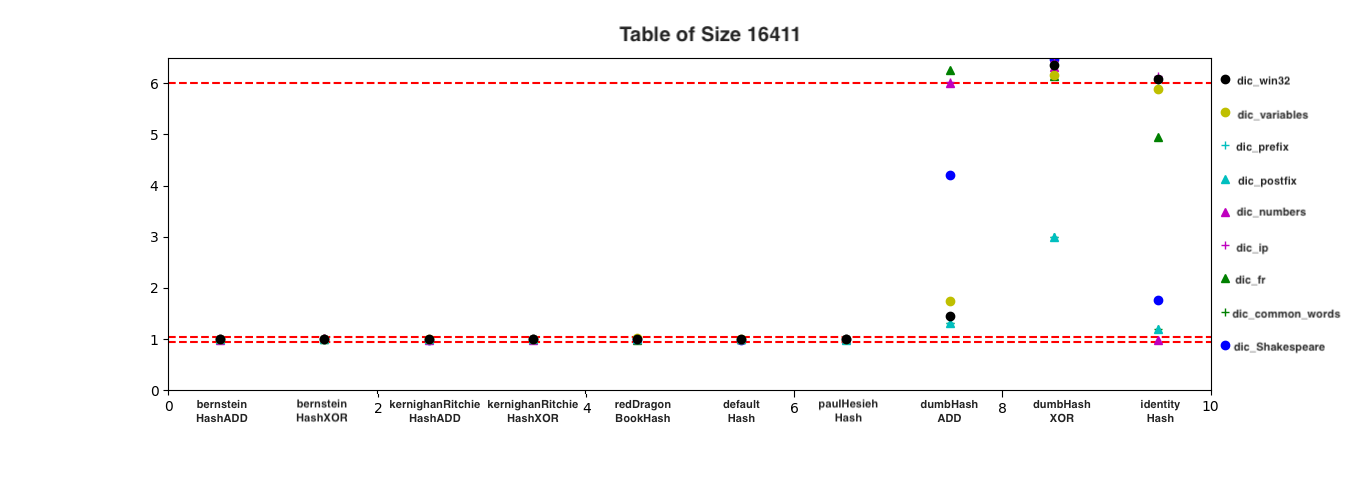
\includegraphics[width=18cm]{figuras/16411HashFunc.png}
  \caption{Functions tested against a ``medium'' sized table}
\end{figure}

\medskip

\begin{figure}[h!]
  \raggedleft
  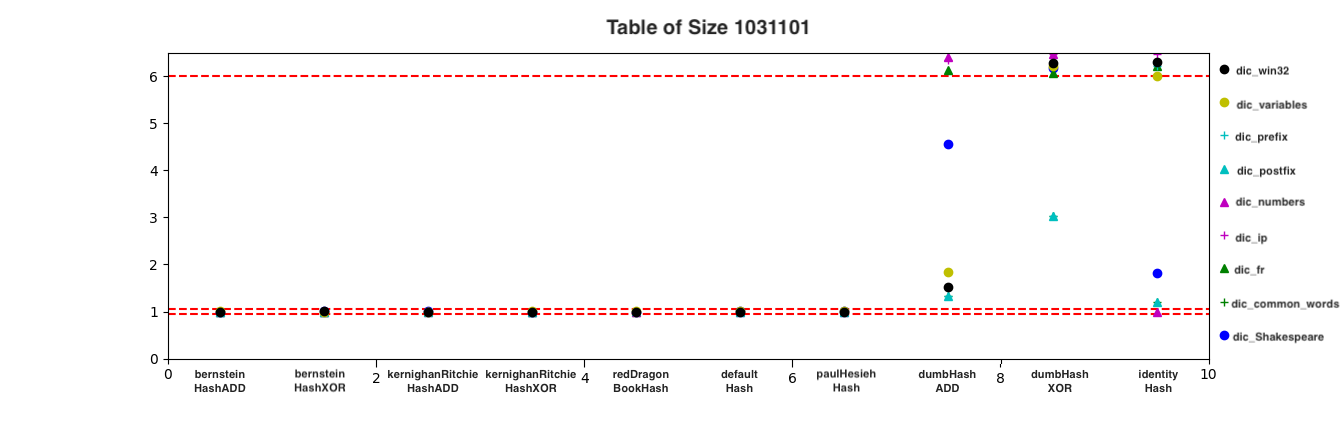
\includegraphics[width=18cm]{figuras/1031101HashFunc.png}
  \caption{Functions tested against a ``large'' table}
\end{figure}

\medskip

The results are shown in the same way displayed in the Red Dragon Book, with Hash functions in the X axis and the ratio displayed in the y axis, with different identification for each file. I choose 3 sizes of tables to count collisions, a ``small'', ``medium'' and a ``large'' table, the small table having a load factor (The percentage of the table occupied) of approximately \( \sim 0.5 \), the medium with \( \sim 0.05 \) and large with \( \sim 0.005 \). It's assumed that the modulo is not the responsaibility of the hash funciton, so all hash functions return values from 0 to \( 2^{32} - 1 \), and the modulo is taken depending on the size of the table. From that we can already see that the load factor doesn't make a good hash function bad, but expose problems of ``bad'' hash functions in some cases. 

Antoher thing that it is important to notice from the graph is the red dotted lines. The top one is the ``Upper'' threshold, which results greater than 6 are just considered ``Big'', as in some cases the ration exploded to values up to 200. The lower 2 red lines are in \( y = 1.05 \) and \( y = 0.95 \) which is the interval that we consider a hash function to have ``Good'' values. 

The tests were made with 10 different hash functions, tested against 9 different files (Provided by strchr website). All of the code used to test this can be found in the github repo \cite{GithubRepo}. The 10 hash functions are the following:

\begin{itemize}
\item \textbf{bernsteinHashADD}: The bernstein hash function described earlier. We use the given hash template adding the elements. The multiplier is 33 and initial value is 5381. In the end we XOR the bits of the hash with itelf shifted 16 to the right (That is half of the bits with our implementation).
  
\item \textbf{bernsteinHashXOR}: The same as above but substituting the first adding operator by the XOR operation.

\item \textbf{kernighanRitchieHashADD} The Kernighan Ritchie Hash function described earlier. We use the given hash template adding the elements. The multiplier is 31 and initial value is 0.

\item \textbf{kernighanRitchieHashXOR} The same as above but substituting the first adding operator by the XOR operation.

\item \textbf{redDragonBookHash} The hash function tested in the red dragon book. It is described as x65599 in the book.

\item \textbf{defaultHash} The default hash function of c++ standard template library.

\item \textbf{paulHesiehHash} A fast hash function described by Paul Hesieh. It is fast to calculate and more complex than Knuth multiplicative or division Hashing.
  
\item \textbf{dumbHashADD} A hash function that simply add all characters.

\item \textbf{dumbHashXOR} A hash function that simply XOR all characters.

\item \textbf{identityHash} A hash function that takes the first 4 bytes of the string.  
\end{itemize}

We have a variety of hash functions, with all being considered ``fast'' hash functions. The files tested inlcude common words in english and french, strings of some IP values, numbers, common variable names and words with common prefix and posfix.

First thing we can notice from those graphs is that changing the ADD function to XOR doesn't make a good mulitiplicative hash function bad. Both are actually ``Equivalent'' given that we are also multiplying the values. For ``dumbHashADD'' and ``dumbHashXOR'' we can see clear differences, with ``dumbHashXOR'' being clearly worse. This can be explained by the cancelation property of XOR. We can see this example on the hash of this IP below:

\[ dumbHashXOR("168.1.1.0") = dumbHashXOR("168.2.2.0") = dumbHashXOR("124.6.8.0") \]

We can see that many different IPs hve the same hash value. More than that, XOR don't increase the number of bits, so all the hashes will be of just 1 byte.

Other thing that we can notice is that ``identity'' hash is good or perfect in some cases. One obvius case that ``identity'' work perfectly is for numbers (We will have 0 collisions). Some languages, like python 3, use the identity function to calculate hash for integers, as it is very fast and produces no collisions. But we can see that for other cases, such as common prefix, it works terrible as we just get the first 4 bytes.

The most common multiplicative hash functions tend to work similarly well, being reasonably close to the ideal hash function in all cases.

As we can see, we don't need a lot of complexity to make a good hash function for a hash table. We have some functions working better for some specific case, like identity function working well for numbers, but general functions already work well enough.

One thing that is important to say here is that hash function is a very vast topic, and here we just covered hash functions related to hash tables. Hash functions have applications in distributed systems (With consistent hashing), database indexing, caching, compilers (As it is explored in the red dragon book) and criptography. Each application has different requirements and make some hash functions better than others.